    %------------------第二章---------------------------
    \newpage
	\section{超声波接近传感器总体设计}

	在进行传感器各部分的设计之前,首先进行整体的设计,如图\ref{超声波接近传感器整体设计}所示,可将超声波接近传感器的设计分为三个大部分:硬件设计、软件设计、实验设计。
\begin{figure}[ht]
	    \centering
	    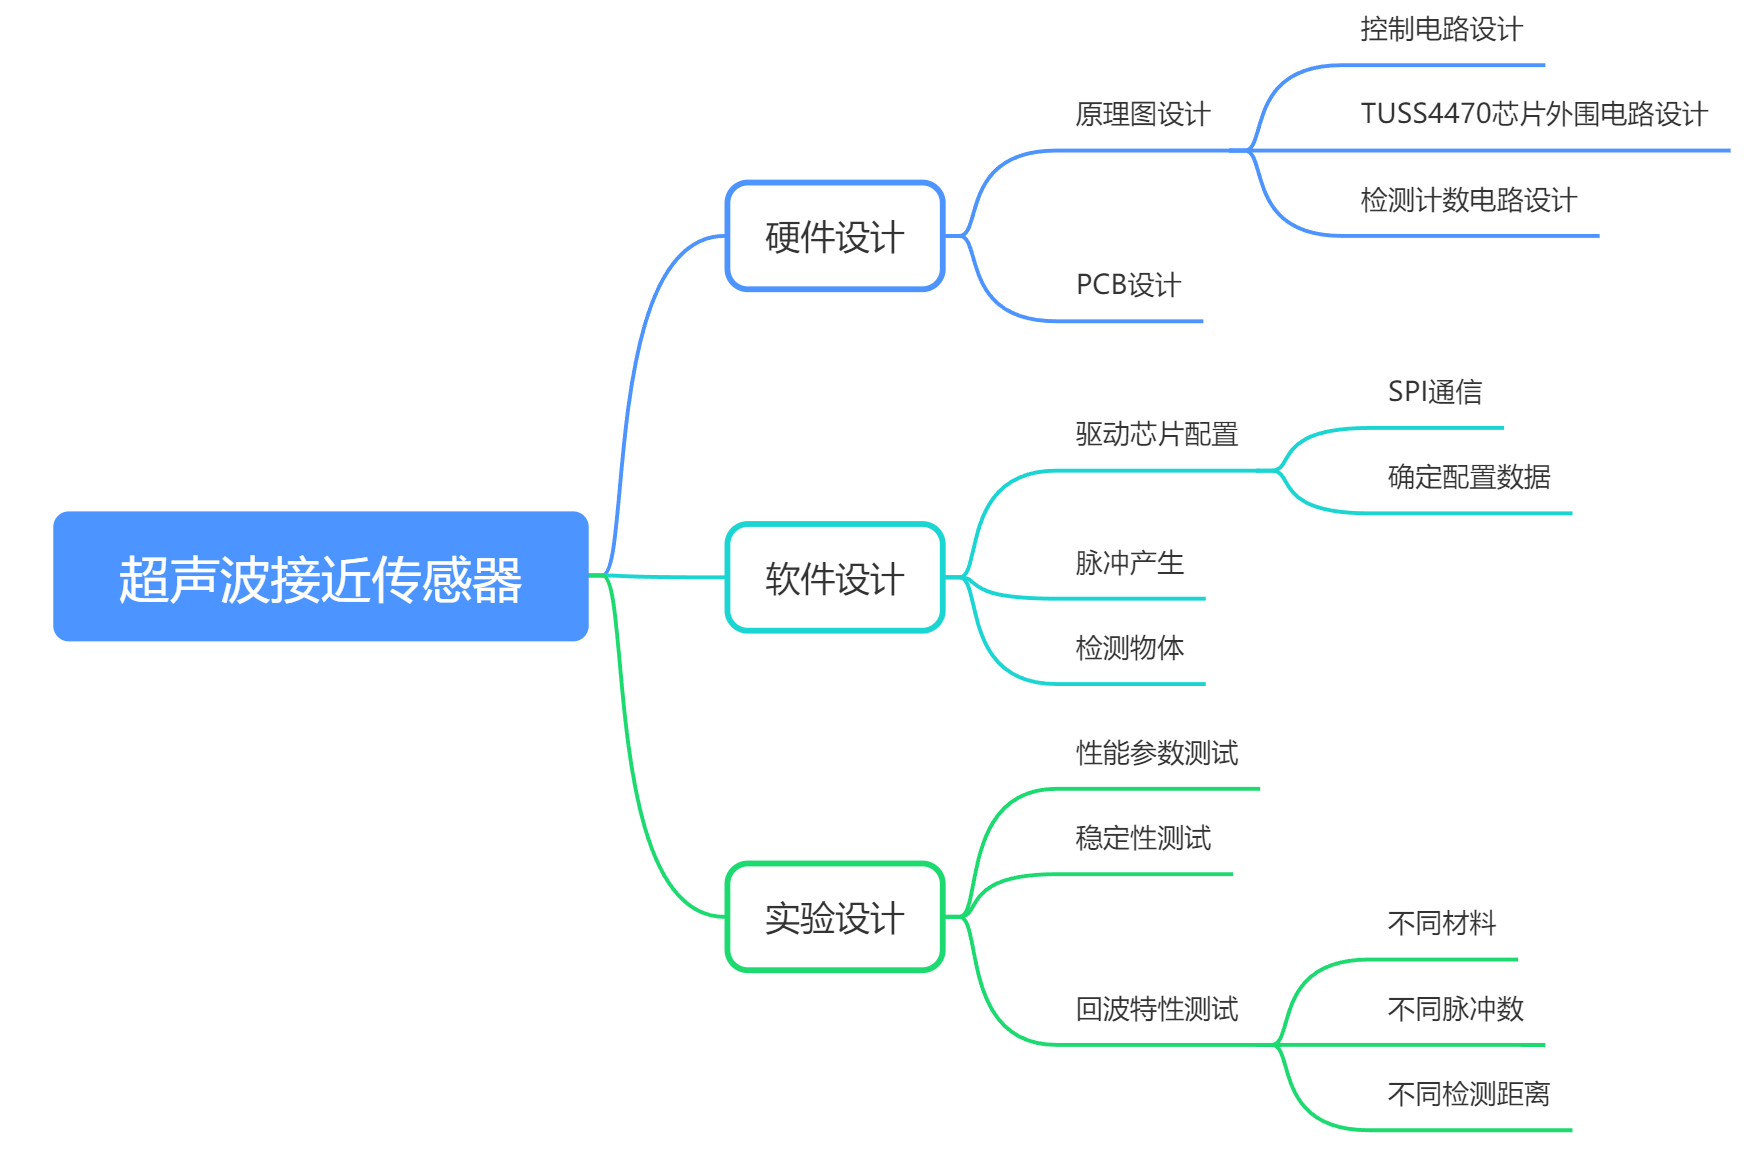
\includegraphics[width=12cm]{figure/overall designment.png}
	    \caption{超声波接近传感器整体设计}
	    \label{超声波接近传感器整体设计}
\end{figure}

 \subsection{超声波接近传感器硬件设计}
硬件电路原理图的设计主要分为三部分来进行,分别为:超声波接近传感器控制电路设计、TUSS4470芯片外围电路设计、检测计数电路设计。其中超声波接近传感器控制电路的设计又包括了电源电路设计、时钟电路设计、JTAG下载电路设计、复位电路设计等。其中设计难度较大的是TUSS4470芯片外围电路,需要通过查阅芯片手册来完成各个引脚的设计。\par
硬件电路的PCB设计在传感器设计中同样有着重要的作用,对于TUSS4470芯片外围电路的PCB设计,芯片手册根据优先级给出了几大原则,用于减小各类信号相互之间的干扰,包括了电容、二极管等器件摆放位置优先级,分离接地,铺铜规则等。
\subsection{超声波接近传感器软件设计}
 超声波接近传感器的软件设计根据功能分为了三个部分:芯片配置、脉冲产生、物体检测。\par
 通过查找芯片手册,可以得知TUSS4470超声驱动芯片采用四线SPI协议来完成芯片配置,并与MCU进行通信,其采用的模式为CPOL=0、CPHA=1,即上升沿进行数据发送、下降沿进行数据接收,根据查找到的资料,本设计采用线性序列机(linear sequential machine)控制移位寄存器俩实现SPI通信。此外,SPI发送的各寄存器配置数据也需要参照芯片手册,根据应用场景进行确认。\par
 在脉冲信号的模式选择上,考虑程序设计的难度以及运行速度,本设计选取脉冲模式3来产生脉冲控制信号,即以io2引脚输入的信号作为时钟信号,io1引脚的下降沿作为脉冲开始的触发信号,上升沿作为脉冲结束的触发信号。程序通过io1、io2引脚信号的下降沿进行触发计数,来得到脉冲信号的脉冲数以及发射次数。\par
 物体检测部分程序主要功能为对回波信号进行处理判断。超声探头发出的脉冲波经物体反射后,重新被传感器所接收,回波信号通过TUSS4470芯片的解调放大处理后,变为简单的回波信号,程序按照检测逻辑对回波信号进行检测判断,从而控制检测状态的转移。
\subsection{超声波接近传感器实验设计}
 在完成实物的制作与调试后,还需要设计实验来测试传感器的性能以及检测逻辑的可行性。\par
 实验设计部分包括了设计实验测试超声波接近传感器性能参数、稳定性以及回波特性。性能参数测试包括了检测范围测试和精度测试,稳定性测试的目的在于测试传感器检测逻辑的必要性,回波特性测试则是为后续的应用提供参考。
 
 